
\documentclass[a4paper, 12pt, twoside, headsepline=true]{scrartcl} % headsepline ist für die Linie unter der Kopfzeile verantwortlich

% Package für Sprachformatierung und Spellchecks
% http://ctan.space-pro.be/tex-archive/macros/latex/contrib/polyglossia/polyglossia.pdf
\usepackage{polyglossia}
\setdefaultlanguage[spelling=new]{german}

% Package zum Ändern von Headern & Footers
% mirrors.ctan.org/macros/latex/contrib/koma-script/doc/scrguien.pdf
\usepackage[automark]{scrlayer-scrpage}
\clearpairofpagestyles
\ihead{\headmark}
\ohead{\pagemark}

\pagestyle{scrheadings}
\setkomafont{pageheadfoot}{\small}

% Package zum Festlegen von Zeilenabstand
% https://www.namsu.de/Extra/pakete/Setspace.html
\usepackage[onehalfspacing]{setspace}
\setmainfont{Charis SIL} % set the main body font (\textrm), assumes Charis SIL is installed
\setlength{\parindent}{0pt}


\usepackage{csquotes}

% Package für das Referenzieren von Quellen aus .bib-Datei
\usepackage[style=ieee]{biblatex}
\addbibresource{mybib.bib}

% Package zum "Patchen" von Befehlen
% http://vesta.informatik.rwth-aachen.de/ftp/pub/mirror/ctan/macros/latex/contrib/xpatch/xpatch.pdf
% Überschreibt biblatex-Funktionalität, damit keine leeren Jahresklammern gedruckt werden
\usepackage{xpatch}
\xpatchbibdriver{online}
{\printtext[parens]{\usebibmacro{date}}}
{\iffieldundef{year}
	{}
	{\printtext[parens]{\usebibmacro{date}}}}
{}
{\typeout{There was an error patching biblatex-ieee (specifically, ieee.bbx's @online driver)}}

% Package zum Anpassen von enumerations-items 
% https://de.wikibooks.org/wiki/LaTeX-W%C3%B6rterbuch:_enumitem
\usepackage{enumitem}
\renewcommand{\labelitemiii}{$\star$}

% Package für die Anpassung der Seitengestaltung, z.B. Seitenränder
% https://www.namsu.de/Extra/pakete/Geometry.html
\usepackage{geometry}

% Package für Tabellengestaltung mit horizontalen Trennlinien
% https://www.namsu.de/Extra/pakete/Booktabs.html
\usepackage{booktabs}

% Package für Gestaltung und Anpassung einzelner Tabellenzellen 
% http://babyname.tips/mirrors/ctan/macros/latex/contrib/makecell/makecell.pdf
\usepackage{makecell}

% Package für Positionierung von "floats", also nichtfesten Elementen wie Tabellen oder Bildern, die sich je nach Textgestaltung verschieden auf der Seite befinden müssen
% http://vesta.informatik.rwth-aachen.de/ftp/pub/mirror/ctan/macros/latex/contrib/float/float.pdf
\usepackage{float}

% Package für Tabellengestaltung 
% https://www.namsu.de/Extra/pakete/Tabularx.html
\usepackage{tabularx,ragged2e}
\newcolumntype{L}{>{\RaggedRight\arraybackslash}X}

% Package zum Anpassen von Macros/KeyValue-Daten. Hab ich garnicht verwendet, glaube ich
% http://mirrors.ibiblio.org/CTAN/macros/latex/contrib/adjustbox/adjustbox.pdf
\usepackage[export]{adjustbox}

% Package für Verwaltung von Acronymen 
% https://www.namsu.de/Extra/pakete/Acronym.html
\usepackage[printonlyused]{acronym}

% Package zum Implementieren von Textlinks
% https://www.namsu.de/Extra/pakete/Hyperref.html
\usepackage[
german,
colorlinks=true,
linkcolor=blue, % einfache interne Verknüpfungen
%TODO: Folgende Zeile für Druckdokument verwenden!
%hidelinks=true
anchorcolor=black,% Ankertext
citecolor=green, % Verweise auf Literaturverzeichniseinträge im Text
urlcolor=cyan % Farbe der URLs
%Back-Links zu den Kapiteln
]{hyperref}
\apptocmd{\UrlBreaks}{\do\f\do\m}{}{}
\setcounter{biburllcpenalty}{9000}% Kleinbuchstaben
\setcounter{biburlucpenalty}{9000}% Großbuchstaben
\setcounter{biburlnumpenalty}{9000}% Zahlen
%\usepackage[german,draft]{hyperref}

%Neudefinition für den Name von Subsubsection, damit "Unterunterabschnitt" nicht bei Referenzen auftaucht
\def\subsubsectionname{Unterabschnitt}%
\def\subsubsectionautorefname{Unterabschnitt}%

% Package für besseren Umgang mit Grafiken
% http://ftp.gwdg.de/pub/ctan/macros/latex/required/graphics/grfguide.pdf
\usepackage{graphicx}

% Package für Platzieren von Bildern neben/im Text
% https://www.namsu.de/Extra/pakete/Wrapfig.html
\usepackage{wrapfig}
\newcommand{\myhline}{\noalign{\global\arrayrulewidth0,1cm}\hline
	\noalign{\global\arrayrulewidth1pt}}
% Umbenennung der Caption Beschreibung unter Bildern von "Abbildung" in "Abb." um Platz zu sparen.
\addto\captionsgerman{%
	\renewcommand{\figurename}{Abb.}%
}

% Definiere eine neue Liste bei der die Unterpunkte auch nummeriert sind, wie bei einem Inhaltsverzeichnis.
\newlist{legal}{enumerate}{10}
\setlist[legal]{label*=\arabic*.}
%\setcounter{tocdepth}{4}
%\setcounter{secnumdepth}{4}

\makeatletter 
\@addtoreset{figure}{section} 
\@addtoreset{table}{section} 
\makeatother 

%Commands zum Neustarten der Seitennummerierung ab Inahltsverzeichnis, falls vorher noch Titelseiten o.Ä. folgen
\renewcommand{\thefigure}{\thesection.\arabic{figure}} 
\renewcommand{\thetable}{\thesection.\arabic{table}} 

\begin{document}
% Nötig um in der PDF Datei einen Lesezeicheneintrag für das Inhaltsverzeichnis zu bekommen.
\pdfbookmark[1]{Inhaltsverzeichnis}{toc}
\tableofcontents
\clearpage
\newpage

\addsec{Abkürzungsverzeichnis}

\pdfbookmark[2]{Abkürzungsverzeichnis}{toc}
% Angabe in eckigen Klammern sollte das längste Acronym enthalten.
% Das ist notwendig damit sich der Einschub am längsten Acronym orientiert.
\begin{acronym}[header=Abkürzungsverzeichnis]
	\acro{bpd}[BPD]{Business Process Diagram}
	\acro{bpel}[BPEL]{Business Process Execution Language}
	\acro{bpm}[BPM]{Business Process Management}
	\acro{bpmn}[BPMN]{Business Process Model and Notation}
	\acro{bpmn4cps}[BPMN4CPS]{Business Process Model and Notation for Cyber-Physical Systems}
	\acro{cmmn}[CMMN]{Case Management Model and Notation}
	\acro{cps}[CPS]{Cyber-Physical Systems}
	\acro{eoi}[EoI]{Entity of Interest}
	\acro{iot}[IoT]{Internet of Things}
	\acro{iota}[IoT-A]{Internet of Things - Architecture}
	\acro{m2m}[M2M]{Machine-to-Machine}
	\acro{omg}[OMG]{Object Management Group}
	\acro{rfid}[RFID]{Radio-frequency Identification}
	\acro{uml}[UML]{Unified Modelling Language}
\end{acronym}

\clearpage

\addcontentsline{toc}{section}{Tabellenverzeichnis}

\listoftables

\clearpage

\addcontentsline{toc}{section}{Abbildungsverzeichnis}
\listoffigures
\clearpage


\section{Einleitung} \label{sec:section}

%TODO Irgendwo einbauen "Ein Workflow ist die informationstechnische Realisierung" Quelle: modelleriungsvorlesung kap 2.1
eines Geschäftsprozesses

\subsection{Motivation} \label{sec:subsection}
Das \ac{iot} ist eines der größten IT-Buzzwords der letzten Jahre und beschreibt die durch eingebettete Elektronik ermöglichte Vernetzung von physischen Dingen. Die dadurch gewonnen Daten bzw. Ereignisse bieten neben dem Potential der
Prozessoptimierung und Erweiterung noch die Möglichkeit zur Generierung völlig neuer Geschäftsprozesse und Modelle. 
Das Weiteren sinken die Kosten dafür physische Dinge mit Sensoren auszustatten und untereinander zu vernetzen, was zu einer hohen Anzahlvon \ac{iot} Projekten führt. Laut Gartner sollen im Jahr 2020 mehr als die Hälfte der wichtigsten Geschäftsprozess Elemente des \ac{iot} beinhalten \cite{garnteriotgrowth}. Da der Wettbewerb auf dem Technologiemarkt rasant zu nimmt, ist es unerlässlich sich von der Konkurrenz abzuheben. Die Verwaltung von von IoT Geräten, sogenannten Smart Devices, mit \ac{bpm} ermöglicht eine einfache Wartung ihrer Orchestrierung. Des weiteren bietet es auch die Möglichkeit der Nachverfolgung, die es ermöglicht KPIs über die Prozesse und Devices einfach zu ermitteln. Diese KPIs sind maßgebend für ein effektives Arbeiten mit der stetig wachsenden Anzahl von Devices \cite{bpmofthings}.

\subsection{Problemstellung} 
Während sich das IoT im Allgemeinen auf Kommunikation und Datenfluss konzentriert, berücksichtigen \ac{bpm}-Ansätze den Kontrollfluss, große monolithische Prozessmodelle und synchrone Interaktionen. Darüber hinaus haben die meisten BPM-Ansätze Probleme mit nicht routinemäßigen, nicht deterministischen Prozessen, während IoT-Anwendungen typischerweise solche Interaktionen beinhalten. Das Problem der Vereinigung von \ac{iot} und \ac{bpm} beginnt bereits bei der Darstellung und Modellierung der neuen Geschäftsprozesse, da Standards wie \ac{bpmn} nur bedingt hierfür geeignete Elemente vorsehen. Das aufkommen der überwältigenden Datenmenge sorgt dafür dass Objekte selbständige Routinen, sogenannte Verhaltensmuster oder Gewohnheiten ausführen. Dieses selbständige Handeln ohne zentrale Steuerung macht die Modellierung umfassender end-to-end Prozesse praktisch unmöglich. Dementsprechend müssen diese Verhaltensmuster als sogenannte event-driven micro processes organisiert werden.Da die Wechselwirkungen zwischen diesen Mikroprozessmodellen nicht auf der niedrigen Ebene des Nachrichtenaustausches beschrieben werden können, müssen diese laut "The Internet-of-Things Meets Business Process Management: Mutual Benefits and Challenges" auf einer höheren semantischen Ebene beschrieben werden \cite{iotmeetsbpm}. Diese Problemstellungen bilden die Grundlage für diese Thesis.

\subsection{Zielsetzung}
Ziel der Thesis ist die Konzeption eines Modellierungsansatzes für \ac{iot}
Workflows. Hierfür werden grundlegende Besonderheiten von \ac{iot} Workflows festgehalten und davon ausgehend Evaluierungskriterien für die Bewertung gängiger Modellierungsansätze abgeleitet. Anhand der Kriterien werden Modellierungsmethoden bewertet und gegebenenfalls mögliche Erweiterungsmöglichkeiten vorgestellt. Der daraus resultierende Ansatz wird auf vorhandene Use-Cases angewandt und bewertet.

\subsection{Aufbau der Thesis}
Nach der Einleitung mit Motivation, Problemstellung, Zielsetzung sowie dem Aufbau der Thesis folgen Grundlagen im Bereich des \ac{iot}, der Prozess Modellierung, des \ac{bpm}, der \ac{iota} sowie der \ac{bpmn4cps}, welche zum Verständnis der weiteren Arbeit dienen.
 
 Im Hauptteil werden typische Muster von \ac{iot} Workflows identifiziert. Aus den identifizierten Workflows werden Unterschiede und Besonderheiten zwischen \ac{iot} Workflows und Workflows ohne \ac{iot} Integration herausgearbeitet, welche bei der Modellierung zu berücksichtigen sind.
 Anhand der Unterschiede werden Evaluierungskriterien für die Geschäftsprozess Modellierung abgeleitet. Diese Evaluierungskriterien werden im Anschluss dazu verwendet um bestehende Modellierungsmethoden auf ihre Eignung zur Modellierung von \ac{iot} Workflows zu bewerten. Basierend auf der Bewertung wird ein Modellierungskonzept für \ac{iot} Workflows erarbeitet. Zur Evaluierung werden mehrere Use-Cases analysisiert und das entwickelte Modellierungskonzept darauf angewandt. Anhand der Ergebnisse wird das Modellierungskonzept bewertet.
 
Im Schlussteil wird das Ergebnis festgehalten, ein Fazit getroffen und weiterführende Arbeiten sowie ein Ausblick vorgestellt.
 
\newpage

\section{Grundlagen} \label{sec:section2}
In diesem Kapitel werden zunächst Grundlagen des \ac{iot} erläutert. Anschließend werden die wichtigsten Prozess Modellierungsmethoden dargestellt und Grundlagen des \ac{bpm} erklärt. Zum Abschluss werden zwei Erweiterungen von \ac{bpmn} zur Modellierung von \ac{iot} Workflows vorgestellt.

\subsection{BPM}
%TODO Übersetzten, ergänzen
Business Process Management (BPM) is a discipline involving any combination of modeling, automation, execution, control, measurement and optimization of business activity flows, in support of enterprise goals, spanning systems, employees, customers and partners within and beyond the enterprise boundaries

BPM is not a product - There is a category called “BPMS” which is a BPM Suite or BPM System.  Gartner has introduced a new product category called “intelligent BPMS.”   What is included depends very much on the vendor. 
%Quelle:https://bpm.com/what-is-bpm

Intelligent BPM:
As a result, we are now moving into a phase that some people are calling “Intelligent BPM Systems,” which is distinguished primarily by the concept of a “sense and respond” capability.   In this way we can see BPM software market in terms of three phases, with each building on the other.
%Quelle: http://data-informed.com/what-big-data-means-to-bpm-more-event-sensors-process-simulations/

\subsection{Internet of Things}

Die Idee eines Internets der Dinge hat seine Ursprünge in den Konzepten des Anfang der 90er Jahre von Mark Weiser skizzierten "Ubiquitous Computing "was er als nahtlose Einbindung von Computern in die reale Welt bezeichnet \cite{ucweiser}. 
Grundgedanke des "Ubiquitous Computing" ist eine Erweiterung beliebiger physischer Gegenstände über ihre bestehende Form und Funktion hinaus durch mikroelektronische Komponenten \cite{237456}. Die so entstehenden"smarten" Gegenstände bilden, mit digitaler Logik, Sensorik und der Möglichkeit zur Vernetzung ausgestattet, ein Internet der Dinge. Der Begriff \acl{iot} selbst wurde jedoch erst 1999 von Kevin Ashton im Zusammenhang eines globalen Netzwerks von Objekten welche mit RFID angereicht wurden bei einer Präsentation bei Procter \& Gamble verwendet \cite{rfidiot}. Eine einheitliche Definition des \ac{iot} gibt es nicht, diese Thesis beruht auf der 2012 publizierten Definition aus "Overview of the IoT" der International Telecommunication Union. Diese definiert \ac{iot} als :"Eine globale Infrastruktur für die Informationsgesellschaft, die fortschrittliche Dienste ermöglicht, indem sie (physische und virtuelle) Dinge miteinander verbindet, die auf bestehenden und sich entwickelnden interoperablen Informations- und Kommunikationstechnologien basieren" \cite{iotdefinition}.
Aus technischer Sicht steht hinter dem Internet der Dinge weniger eine einzelne Technologie oder eine spezifische Funktionalität als vielmehr ein Funktionsbündel, welches in seiner Gesamtheit eine neue Qualität der Informationsverarbeitung entstehen lässt und somit neue Geschäftsmodelle ermöglicht.

\subsubsection{Smart Objects}
 Die in Tabelle \ref{table:smartObjectsCharacteristics} auf Seite \pageref{table:smartObjectsCharacteristics} sichtbaren charakteristischen Merkmale unterscheiden die "smarten" Objekte des \ac{iot} zwischen Objekten welche nicht Teil des \ac{iot} sind.

\begin{table}[H]
	\begin{tabularx}{\textwidth}{@{}lL@{}} 
		\toprule
		\textbf{Charakteristik} & \textbf{Erklärung} 
		\\ \midrule
		Identifikation & Objekte im Internet der Dinge sind über einen Schlüssel eindeutig identifizierbar. Diese Identifikation ermöglicht die Verknüpfung des Objekts mit Diensten, welche Informationen des physischen Objektes auf einem Server bereitstellen. 
		\\ \hline
		Kommunikation & Im Gegensatz zu herkömmlichen phyischen Objekten verfügen Objekte im Internet der Dinge über die Möglichkeit Ressourcen im Netz oder sogar untereinander zur Verfügung zu stellen, um Daten und Dienste gegenseitig zu nutzen.
		\\ \hline
		Sensorik & Das "smarte" Objekt sammelt Informationen über seine Umwelt (Temperatur, Lichtverhältnisse, Luftdruck usw.), zeichnet diese auf und/oder reagiert darauf
		\\ \hline
		Lokalisierung & Smarte Objekte kennen ihren Aufenthaltsort oder sind für andere lokalisierbar, bspw. auf globaler Ebene durch GPS oder in Innenräumen durch Ultraschall 
		\\ \hline
		Speicher & Das Objekt verfügt über Speicherkapazität, so dass es beispielsweise. Informationen über seine Vergangenheit mit sich tragen kann
		 \\ \hline
		Aktuatorik & Objekte im Internet der Dinge können unter Umständen selbständig Entscheidungen ohne übergeordnete Planungsinstanz treffen, z.B. im Sinne eines Industriecontainers, der seinen Weg durch die Lieferkette selbst bestimmt
		\\ \hline
		Benutzerschnittstelle & Mit dem Aufgehen des Computers im physischen Gegenstand stellen sich auch neue Anforderungen an die Benutzeroberfläche, die meist nicht mehr durch Tasten und Displays realisiert werden kann. Vielmehr braucht es hier neuartige Benutzungsmetaphern analog der Maus und Fenstermetapher graphischer Benutzeroberflächen
		\\ \hline
		\bottomrule
	\end{tabularx}
\caption{Charakteristiken von "smarten" Objekten\cite{iotwiki}}
\label{table:smartObjectsCharacteristics}
\end{table}

%TODO Tabelle über zwei seiten

\subsubsection{Domain Model}

Da es unter der Buzzword \ac{iot} sehr viele unterschiedlich Auffassungen und Interpretation wie zum Beispiel das ursprüngliche Konzept Kevin Ashtons eines Netzwerkes um RFID angereicherte Objekte. Häufig ist auch von \ac{m2m} oder \ac{cps} die Rede. Bei dieser Vielzahl von Auffassungen und Begriffen ist es für ein allgemeines Verständnis unabdingbar sich auf eine Definition zu einigen. Im Zuge dieser Thesis wird das 2010 von Stephan Haller vorgestellte IoT Domain Model verwendet um den Zusammenhang zwischen Devices, Resourcen und Services zu erklären\cite{haller2010things}, da diese die am häufigsten verwendetet wurde in der Literatur auf welcher diese Thesis beruht. Die auf Seite \pageref{fig:domainmodel} zeigt eine auf den Zusammenhang von Device, Service und Ressourcen abstrahierte Darstellung des IoT Domain Models. Im Anhang befindet sich ein Schaubild des vollständigen IoT Domain Models Haller´s vom Stand 2013.

\begin{figure}[H]
	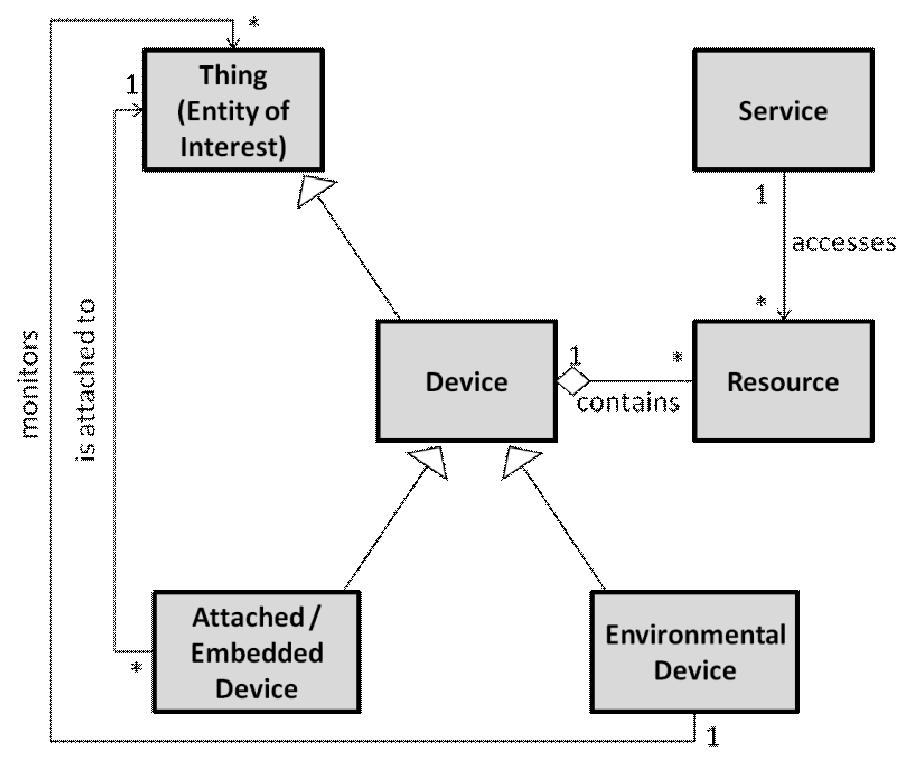
\includegraphics[height=10 cm,keepaspectratio,center]{figures/domainmodel}
	\vspace{0.5cm}
	\caption{Zusammenhang zwischen Thing, Device, Ressource und Service \cite{haller2010things}}
	\label{domainmodel}
\end{figure}

\textbf{Thing/ \ac{eoi}}: \\ 
Das \ac{eoi} bezeichnet einen physischen Gegenstand an welchem der Nutzer oder eine Anwendung wie zum Beispiel ein Geschäftsprozess. Das \ac{eoi} wird entweder durch ein Environmental Device oder über ein "attached" beziehungsweise "embedded device" überwacht.
\\

\textbf{environmental Device}: 
Environmental Devices, also Umgebungsgeräte überwachen und verfolgen den Status des \ac{eoi}. Beispiele für Umgebungsgeräte sind \ac{rfid} Lesegeräte, Barcodescanner oder Kameras

\textbf{attached/ embedded Device}: 
Als attached/embedded Device stellen ähnlich wie die Umgebungsgeräte den Zustand und den Status des \ac{eoi} fest. Der Unterschied liegt hierbei daran, dass die attached/embedded Devices am \ac{eoi} selbst und nicht in der Umgebung angebracht sind. Beispiel hierfür sind Sensoren wie Thermometer oder Manometer.
\\

\textbf{Device}: \\
Das Device wird als Überklasse der "environmental Devices" sowie der "attached/ embedded Device" verstanden und stellt das virtuelle Gegenstück zum \ac{eoi} dar.
\\

\textbf{Resource}: \\
Als werden die vom Device bereitgestellten digitalen Informationen über den Zustand oder die Betätigungsfähigkeiten eines physischen Objektes bezeichnet.
\\

\textbf{Service}: \\
Services stellen die Ressourcen des Devices über eine klar definierte und standardisierte Schnittstelle bereit und stellen sie somit Anwendungen oder anderen Services zur Verfügung. Somit wird die Funktionalität als Arbeitseinheit einem Geschäftsprozess zur Verfügung gestellt.
\\
\\
Zusammenfassend lässt sich der Zusammenhang zwischen \ac{eoi}, Device, Service und Resource also wie folgend beschreiben. Ein physisches Objekte an welchem Interesse besteht wird durch die Überwachung mittels ein oder mehrerer Sensoren beziehungsweise Umgebungsgeräten als Device in der virtuellen Welt dargestellt. Dieses Device enthält mehrere Ressourcen also Informationen welche wiederum durch standardisierte Schnittstellen, den Services zur Verfügung gestellt werden.

\subsection{Prozess Modellierung}

In vielen heutigen Unternehmen unterstützen Informationssysteme nicht mehr nur das Geschäft,sondern sie werden immer mehr zu einem integralen Bestandteil davon. Alle Unternehmen machen Gebrauch von Informationstechnologie, und es ist wichtig, dass ihre Systeme so aufgebaut sind, dass sie die Unternehmen unterstützen in denen sie zum Einsatz kommen. Das Geschäft bestimmt letztlich die Anforderungen, welche die Informationssysteme definieren. Die Entwicklung von Software ohne ein angemessenes Verständnis des Kontextes, in welchem diese Software betrieben werden soll, ist nahezu unmöglich. Um ein solches Verständnis zu erlangen, ist es unerlässlich, dass man ein Geschäftsmodell definiert. Ein Modell ist eine vereinfachte Sicht auf eine
komplexe Realität. Diese Abstraktion erlaubt es irrelevante Details zu vernachlässigen und den Fokus auf die Kernelemente zu legen. Effektive Modelle erleichtern zudem
Diskussionen zwischen verschiedenen Stakeholdern im Unternehmen.
Sie ermöglichen es ihnen, sich auf die wichtigsten Grundlagen zu einigen und auf gemeinsame Ziele hinzuarbeiten. Die Modellierung von Geschäftsprozessen ist als Mittel zur Analyse und zum Design von Software akzeptiert und etabliert. Die sich ständig weiterentwickelnden Modelle helfen den Entwicklern auch dabei, ihr Denken zu strukturieren und zu fokussieren. Die Arbeit mit den Modellen dient ihnen zum Verständnis für das Geschäft und erhöht dadurch das Bewusstsein für neue Möglichkeiten zur Verbesserung des Geschäfts.

\subsubsection{BPMN}

\ac{bpmn} ist ein Standard für die Geschäftsprozessmodellierung, der eine grafische Notation zur Spezifikation von Geschäftsprozessen in einem \ac{bpd} auf Grundlage traditioneller Flussdiagrammtechniken bereitstellt \cite[S.222]{Aagesen2015}. Das Ziel von \ac{bpmn} ist es, die Geschäftsprozessmodellierung sowohl für technische Anwender als auch für Geschäftsanwender zugänglich zu machen,damit die Geschäftsprozessmodellierung eine Kommunikations- und Automatisierungsgrundlage bildet. Hierfür wird eine Notation bereitgestellt wird, welche für Geschäftsanwender intuitiv ist und dennoch komplexe Prozesssemantik abbilden kann. Die seit 2011 von der \ac{omg} vorgestellte \ac{bpmn} 2.0-Spezifikation bietet auch Ausführungssemantik sowie das Mapping zwischen den Grafiken der Notation und anderen Ausführungssprachen, insbesondere der \ac{bpel}. \ac{bpmn} ist so konzipiert, dass es für alle Beteiligten leicht verständlich ist.
Zu den Anwendern gehören Business-Analysten, welche die Prozesse erstellen und verfeinern, technische Entwickler, die für die Implementierung zuständig sind sowie Führungskräfte welche Prozesse überwachen und verwalten \cite{vonRosing2015433}. Im Anhang befindet sich ein Poster mit einer Übersicht über die wichtigsten Modellierungsmethoden von \ac{bpmn}. 


Aufgrund der fehlenden Möglichkeit Flexibilität abzubilden beziehungsweise da nicht alle Möglichen Szenarien bekannt sind oder aufgrund der Kombinatorik nicht modelliert werden können, wurde 2014 von der \ac{omg} ein eigener Standard \ac{cmmn} verabschiedet welcher in der Lage ist flexible Prozesse abzubilden. Als Case wird eine Aktivität bezeichnet, welche sich nicht einfach wiederholen lässt. Cases sind von sich entwickelnden Umständen oder von Ad-hoc-Entscheidungen im Bezug auf bestimmte Situationen abhängig. Diese Ad-hoc-Entscheidungen werden von sogenannten Wissensarbeitern gefällt. Zu den Anwendungsfällen des Case Managements gehören die Antrags- und Schadensbearbeitung in der Versicherungsbranche, die Patientenversorgung sowie die medizinische Diagnose im Gesundheitswesen,
Hypothekenbearbeitung im Bankwesen, Problemlösung in Call Centern, Wartung und Reparatur von Maschinen und Anlagen sowie die Konstruktion von Sonderanfertigungen\cite{cmmnomg} .

Laut Heise sei die Kombination von \ac{cmmn} und \ac{bpmn} sinnvoll um sowohl strukturierte als auch unstrukturierte Prozesse oder Teilprozesse sinnvoll abbilden zu können \cite{cmmnheise}.


\subsubsection{UML}

 \ac{uml} ist eine grafische Sprache, die die Artefakte verteilter Objektsysteme visualisiert, spezifiziert, konstruiert und dokumentiert \cite{Kleuker}. Es ist der am weitesten verbreitete Standard für Software-Architekten, um Geschäftsanwendungen zu spezifizieren. \ac{uml} wird vor allem für die objektorientierte Softwareentwicklung im Bereich des Software-Engineerings eingesetzt.
Die \ac{uml} wurde in den 90er Jahren als Modellierungssprache und Methodik zur Unterstützung der objektorientierten Programmierung entwickelt. Im Jahr 1997 wurde es als Standard von der \ac{omg} übernommen. Die ersten Versionen 1.X wurden 2005 durch die neu überarbeiteten Versionen 2.X ersetzt. Seit März 2015 befindet sich UML in der Version 2.5 \cite{omguml}. \ac{uml} bietet im Gegenteil zu \ac{bpmn} mehr als nur die reine Prozessmodellierung und ist ihrer Gesamtheit sehr Umfangreich. Die Spezifikation allein ist über eintausend Seiten lang. Strukturiert wird \ac{uml} in vier Gruppen, den  Strukturdiagrammen, den Architekturdiagrammen, den Verhaltensdiagrammen und den Kommunikationsdiagrammen%TODO Quelle modellierungsvorlesung kapitel 1.1.
Im Zuge dieser Thesis wird \ac{uml} lediglich auf \ac{uml} Aktivitätsdiagramme im Bezug auf Prozessmodellierung eingegangen.

\subsubsection{Geschäftsregeln}



\subsection{IoT - A}

\subsection{BPMN4CPS}

\newpage

\section{BPM und IoT}		
Obwohl IoT mittlerweile zum beliebten Schlagwort geworden ist, kämpfen viele immer noch mit dem Konzept, Prozesse auf IoT anzuwenden. BPM, in seinem Kern, nutzt den Workflow, um große Daten- und Informationsmengen zu verwalten, zu aktualisieren und zu verfolgen. Wenn zum Beispiel eine intelligente Uhr Daten von Ihrem Handgelenk empfängt, die sie dann an eine Fitness-Überwachungsapplikation überträgt, woher weiß sie dann, was sie mit diesen Informationen zu tun hat? Speichert es die Daten einfach in seinem Speicher? Schickt es die Daten an andere Anwendungen, die Ihre Gesundheit, Ihre Ernährung und Ihren Zeitplan für medizinische Besuche überwachen? Prozesse wie diese nutzen BPM, um intelligente Objekte und Anwendungen in der richtigen Reihenfolge zu verwalten. Das Volumen der Daten, mit denen wir täglich arbeiten, nimmt exponentiell zu, so dass es für uns eine absolute Notwendigkeit ist, diese Informationen in beziehungsweise mit Prozessen besser zu verwalten. BPM erhöht den Wert des IoT durch die Verbindung von intelligenten Objekten. Dies wiederum erweitert ihre Integration und Orchestrierung. Da immer mehr Geräte angeschlossen werden und die IoT-Nutzung zunimmt, besteht eine größere Wahrscheinlichkeit für Chaos, dass durch die schnelle Vervielfältigung einzelner Schnittstellen ausgelöst wird. Intelligente Geräte senden Informationen von einem angeschlossenen Gerät über eine API, um eine Antwort zu aktivieren. Die Antworten können in einem kompletten Prozess orchestriert werden, wobei nachfolgende Antworten wie z.B. das Öffnen einer Autotür oder der systematische Zugriff auf bestimmte Dateien aufgerufen werden. Die Integration von BPM ermöglicht es, viele Dinge innerhalb des IoT richtig und nahtlos zusammen zu managen \cite{bpmofthings} .
% Bessere Stelle für Zitierung finden

\subsection{Typische Muster und Best Practices von IoT Workflows}

\subsection{Unterschiede IoT Workflows zu regulären Workflows}

\subsection{Evaluierungskriterien}

\subsection{Bewertung der Modellierungsmethoden}

\subsection{Modellierungskonzept}

\newpage

\section{Evaluierung}

\newpage

\section{Schlussteil}

\subsection{Ergebnis}

\subsection{Fazit}

\subsection{Weiterführende Arbeit/ Ausblick}

\newpage

\addsec{Literaturverzeichnis}
\printbibliography[heading=none]
\newpage
\addsec{Anhang}
\subsection*{Unterbereich Anhang}
\end{document}
